\section{Auswertung}
\label{sec:Auswertung}
Die Messwerte sind in den Tabellen \ref{tab:messwerte} aufgetragen.
In Abbildungen \ref{fig:uidiagramm1} \ref{fig:uidiagramm2}sind die die gemessenen Bremsspannungen $U_\text{B}$ gegen die Wurzel des Photostroms $I_0$ aufgetragen.

\begin{figure}[p]
	\centering
	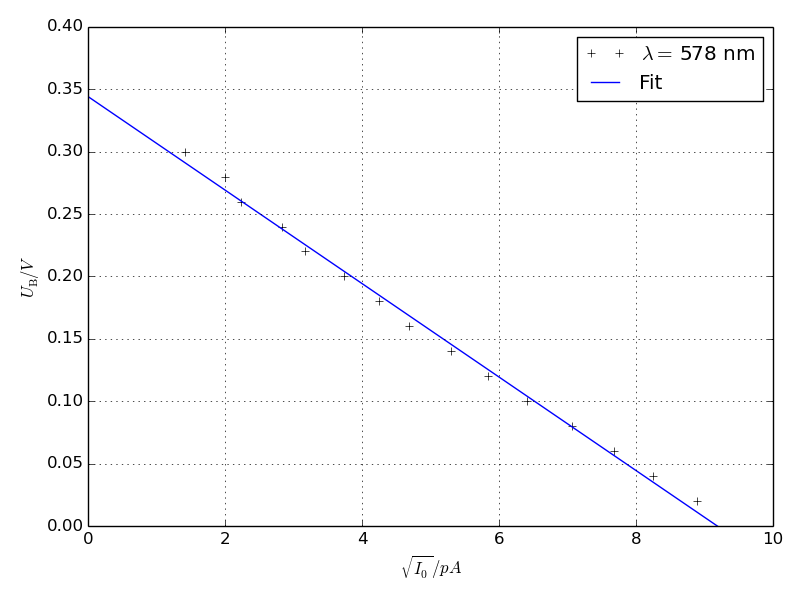
\includegraphics[width=\textwidth]{Bilder/Fit_gelb.png}
	\caption{Gemessene Photostromstärken in Abhängigkeit von den Bremsspannungen, Messung bei gelber Spektrallinie.}
	\label{fig:uidiagramm1}
\end{figure}
\begin{figure}[p]
	\centering
	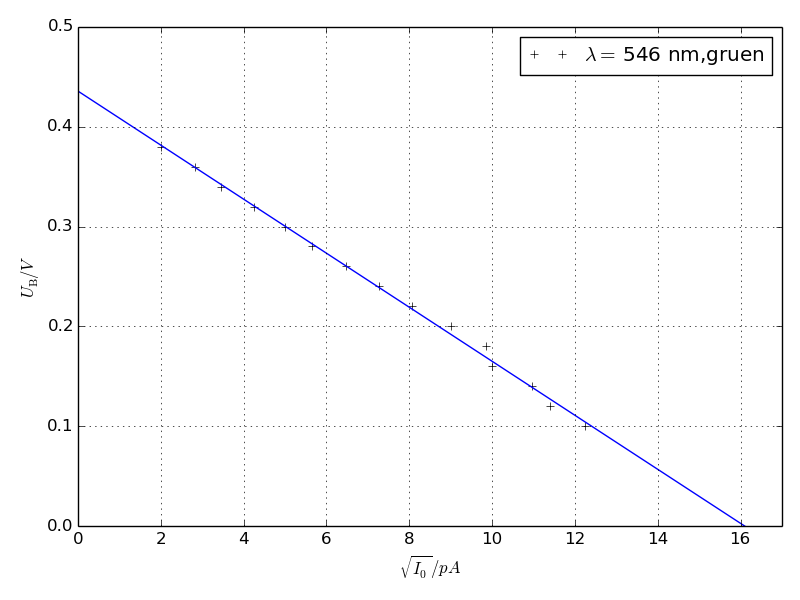
\includegraphics[width=\textwidth]{Bilder/Fit_gruen.png}
	\caption{Gemessene Photostromstärken in Abhängigkeit von den Bremsspannungen, Messung bei grüner Spektrallinie.}
	\label{fig:label}
\end{figure}
\begin{figure}[p]
	\centering
	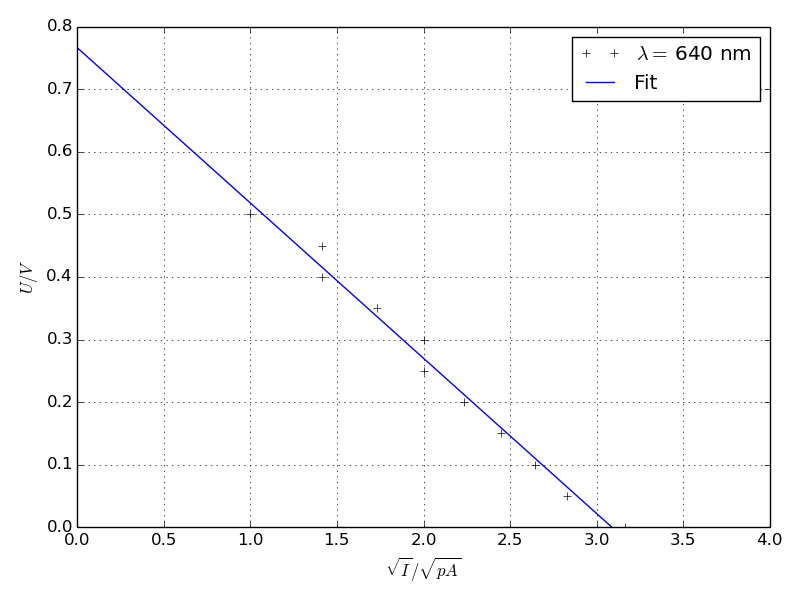
\includegraphics[width=\textwidth]{Bilder/Fit_rot.png}
	\caption{Gemessene Photostromstärken in Abhängigkeit von den Bremsspannungen, Messung bei roter Spektrallinie.}
	\label{fig:label}
\end{figure}
\begin{figure}[p]
	\centering
	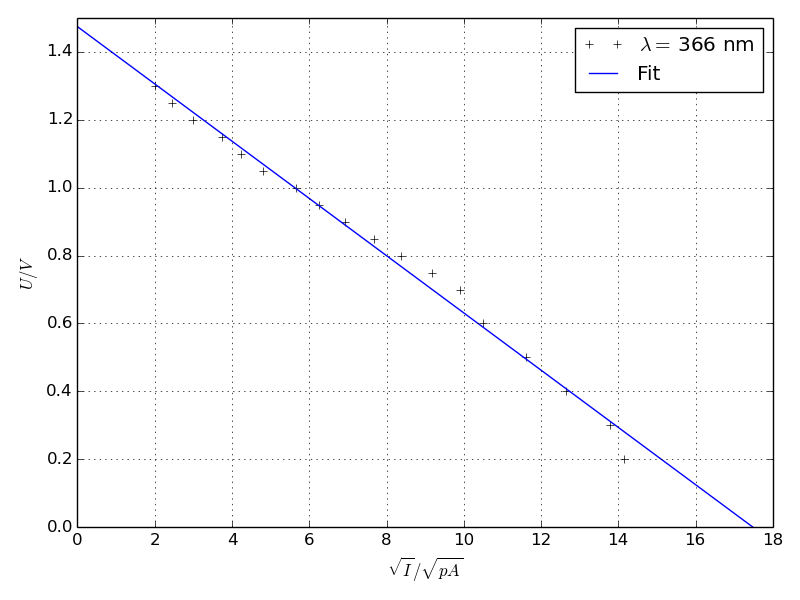
\includegraphics[width=\textwidth]{Bilder/Fit_uv.png}
	\caption{Gemessene Photostromstärken in Abhängigkeit von den Bremsspannungen, Messung bei UV-Spektrallinie.}
	\label{fig:label}
\end{figure}
\begin{figure}[p]
	\centering
	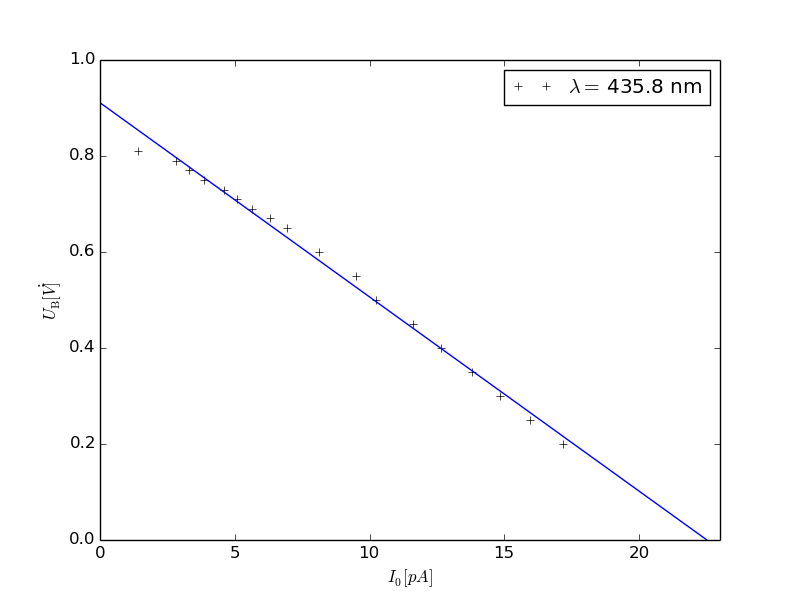
\includegraphics[width=\textwidth]{Bilder/Fit_violett.png}
	\caption{Gemessene Photostromstärken in Abhängigkeit von den Bremsspannungen, Messung bei violetter Spektrallinie.}
	\label{fig:uidiagramm2}
\end{figure}
\begin{landscape}
	\begin{minipage}[c][12cm][t]{0.3\textwidth}
		\centering
		\begin{tabular}{S[table-format=1.2] S[table-format=3.0]}
			\toprule
			\multicolumn{2}{c}{UV-Spektrallinie}\\ 
			\multicolumn{2}{c}{$\lambda=\SI{266.3}{\nano\meter}$}\\
			{$U_\text{B}/\:\si{\volt}$} & {$I_0/\:\si{\pico\ampere}$}\\	
			\midrule
				 0.20 & 200\\
				 0.30 & 190\\
				 0.40 & 160\\
				 0.50 & 135\\
				 0.60 & 110\\
				 0.70 &  98\\
				 0.75 &  84\\
				 0.80 &  70\\
				 0.85 &  59\\
				 0.90 &  48\\
				 0.95 &  39\\
				 1.00 &  32\\
				 1.05 &  23\\
				 1.10 &  18\\
				 1.15 &  14\\
				 1.20 &   9\\
				 1.25 &   6\\
				 1.30 &   4\\
				 1.345&   0\\
			\bottomrule
			\end{tabular}
	\end{minipage}
	\begin{minipage}[c][12cm][t]{0.3\textwidth}
		\centering
		\begin{tabular}{S[table-format=1.2] S[table-format=3.0]}
			\toprule
			\multicolumn{2}{c}{Violette Spektrallinie}\\ 
			\multicolumn{2}{c}{$\lambda=\SI{435.8}{\nano\meter}$}\\
			{$U_\text{B}/\:\si{\volt}$} & {$I_0/\:\si{\pico\ampere}$}\\	
			\midrule
				 0.20&	295\\
				 0.25&	255\\
				 0.30&	220\\
				 0.35&	190\\
				 0.40&	160\\
				 0.45&	135\\
				 0.50&	105\\
				 0.55&	 90\\
				 0.60&	 66\\
				 0.65&	 48\\
				 0.67&	 40\\
				 0.69&	 32\\
				 0.71&	 26\\
				 0.73&	 21\\
				 0.75&	 15\\
				 0.77&	 11\\
				 0.79&	  8\\
				 0.81&	  2\\
				 0.83&	  0\\
			\bottomrule
			\end{tabular}
	\end{minipage}
	\begin{minipage}[c][12cm][t]{0.3\textwidth}
		\centering
		\begin{tabular}{S[table-format=1.2] S[table-format=3.0]}
			\toprule
			\multicolumn{2}{c}{Grüne Spektrallinie}\\
			\multicolumn{2}{c}{$\lambda=\SI{546}{\nano\meter}$}\\
			{$U_\text{B}/\:\si{\volt}$} & {$I_0/\:\si{\pico\ampere}$}\\	
			\midrule
				0.10	&150\\	
				0.12	&130\\
				0.14	&120\\
				0.16	&100\\
				0.18	& 97\\
				0.20	& 81\\
				0.22	& 65\\
				0.24	& 53\\
				0.26 	& 42\\
				0.28	& 32\\
				0.30	& 25\\
				0.32	& 18\\
				0.34	& 12\\
				0.36	&  8\\
				0.38	&  4\\
				0.397	&  0\\
			\bottomrule
			\end{tabular}
	\end{minipage}
	\begin{minipage}[c][12cm][t]{0.3\textwidth}
		\centering
		\begin{tabular}{S[table-format=1.2] S[table-format=3.0]}
			\toprule
			\multicolumn{2}{c}{Gelbe Spektrallinie}\\
			\multicolumn{2}{c}{$\lambda=\SI{578}{\nano\meter}$}\\
			{$U_\text{B}/\:\si{\volt}$} & {$I_0/\:\si{\pico\ampere}$}\\	
			\midrule
				0.02	& 79\\
				0.04	& 68\\
				0.06	& 59\\
				0.08	& 50\\
				0.10	& 41\\
				0.12	& 34\\
				0.14	& 28\\
				0.16	& 22\\
				0.18	& 18\\
				0.20	& 14\\
				0.22	& 10\\
				0.24	& 8\\
				0.26	& 5\\
				0.28	& 4\\
				0.30	& 2\\
				0.32	& 0\\
			\bottomrule
			\end{tabular}
	\end{minipage}
	\begin{minipage}[c][12cm][t]{0.3\textwidth}
		\centering
		\begin{tabular}{S[table-format=1.2] S[table-format=3.0]}
			\toprule
			\multicolumn{2}{c}{Rote Spektrallinie}\\
			\multicolumn{2}{c}{$\lambda=\SI{640}{\nano\meter}$}\\
			{$U_\text{B}/\:\si{\volt}$} & {$I_0/\:\si{\pico\ampere}$}\\	
			\midrule
				0.00	&10\\
				0.05	& 8\\
				0.10	& 7\\
				0.15	& 6\\
				0.20	& 5\\
				0.25	& 4\\
				0.30	& 4\\
				0.35	& 3\\
				0.40	& 2\\
				0.45	& 2\\
				0.50	& 1\\
				0.506	& 0\\
			\bottomrule
			\end{tabular}
	\end{minipage}
\begin{table}[ht]
\caption{Die gemessenen Bremsspannungen \texorpdfstring{$U_\text{B}$}{U} und Photoströme \texorpdfstring{$I_0$}{I}in Abhängigkeit von der Wellenlänge \texorpdfstring{$\lambda$}{} des Lichtes.}
\label{tab:messwerte}
\end{table}
\end{landscape}